%%%%%%%%%%%%%%%%%%%%%%%%%%%%%%%%%%%%%%%%%
% Master's review poster -- Transformer Pruning (state of the art)
% Built on the Jacobs/Dalhousie landscape conference-poster template.
% Content distilled from sections/compression/neural_network_pruning.tex.
%%%%%%%%%%%%%%%%%%%%%%%%%%%%%%%%%%%%%%%%%

\documentclass[final]{beamer}
\usepackage[scale=1.24]{beamerposter}
\usetheme{confposter}

\setbeamercolor{block title}{fg=black,bg=white}
\setbeamercolor{block body}{fg=black,bg=white}
\setbeamercolor{block alerted title}{fg=white,bg=black}
\setbeamercolor{block alerted body}{fg=black,bg=white}

%-----------------------------------------------------------
% Column geometry (4-column basis: one / two / three column widths)
\newlength{\sepwid}
\newlength{\onecolwid}
\newlength{\twocolwid}
\newlength{\threecolwid}
\setlength{\paperwidth}{48in}
\setlength{\paperheight}{58in} % enlarged for now so nothing clips; resize later
\setlength{\sepwid}{0.024\paperwidth}
\setlength{\onecolwid}{0.22\paperwidth}
\setlength{\twocolwid}{0.464\paperwidth}
\setlength{\threecolwid}{0.708\paperwidth}
\setlength{\topmargin}{-0.5in}
%-----------------------------------------------------------

\usepackage{graphicx}
\usepackage{booktabs}
\usepackage{tabularx}
\usepackage{amsmath,amssymb}

% TikZ / pgfplots for the two reused figures
\usepackage{tikz}
\usepackage{pgfplots}
\pgfplotsset{compat=1.18}
\usetikzlibrary{positioning,arrows.meta,calc}

% Colours used by the reused report figures
\definecolor{colBlue}{RGB}{141,180,226}
\definecolor{colBlueBorder}{RGB}{49,112,185}
\definecolor{colGreen}{RGB}{160,215,145}
\definecolor{headergreen}{RGB}{50,180,50}
\definecolor{actred}{RGB}{240,180,180}
\definecolor{actreddark}{RGB}{220,100,100}
\definecolor{slateblue}{HTML}{7A90B2}

% Math shortcuts taken from the report so equations paste verbatim
\newcommand{\R}{\mathbb{R}}
\newcommand{\norm}[1]{\left\lVert #1 \right\rVert}
\DeclareMathOperator{\diag}{diag}

%----------------------------------------------------------------------------------------
\title{Transformer Pruning: From Local Saliency Criteria to Global Configuration Search}
\author{[Author Name]}
\institute{[University / Department] \\[0.5ex] Supervisor: [Supervisor Name]}
%----------------------------------------------------------------------------------------

\begin{document}

\addtobeamertemplate{block end}{}{\vspace*{2ex}}
\addtobeamertemplate{block alerted end}{}{\vspace*{2ex}}
\setlength{\belowcaptionskip}{2ex}
\setlength\belowdisplayshortskip{2ex}

\begin{frame}[t]
\begin{columns}[t]

\begin{column}{\sepwid}\end{column} % spacer

%========================================================================
% COLUMN 1
%========================================================================
\begin{column}{\onecolwid}

%---- Aims (grey alert) ----
\setbeamercolor{block alerted title}{fg=white,bg=dalgrey}
\setbeamercolor{block alerted body}{fg=black,bg=white}
\begin{alertblock}{Aims}
This poster surveys the state of the art in pruning Transformer models and
organises it along three axes:
\begin{itemize}
\item \textbf{What is removed} --- the sparsity topology and the structural unit.
\item \textbf{What drives removal} --- the saliency criterion that estimates a unit's importance.
\item \textbf{How removal is scheduled} --- the pruning strategy and the budget allocation across layers.
\end{itemize}
The recurring limitation of \emph{local}, per-unit scoring motivates a shift
toward \emph{global, budget-constrained configuration search}.
\end{alertblock}

%---- Why prune? ----
\begin{block}{Why Prune Transformers?}
Transformer quality scales with size, but deployment is bounded by memory,
bandwidth, latency, and energy. Pruning reduces the active parameters or
executable units while preserving predictive behaviour, exploiting the
pronounced over-parameterisation of modern models.
\begin{table}
\renewcommand{\arraystretch}{1.2}
\small
\begin{tabularx}{\linewidth}{lrrX}
\toprule
\textbf{Model} & \textbf{Params} & \textbf{FP16 (GB)} & \textbf{Type} \\
\midrule
ResNet-50      & 25.6 M & 0.05 & Vision \\
BERT-Base      & 110 M  & 0.22 & Encoder LM \\
GPT-2 (XL)     & 1.56 B & 3.12 & Decoder LM \\
LLaMA-2 (7B)   & 6.74 B & 13.5 & Open LLM \\
LLaMA-2 (70B)  & 68.9 B & 138  & Multi-GPU \\
\bottomrule
\end{tabularx}
\caption{Parameter counts and FP16 memory footprints. Even at 50\% sparsity a
70B model still needs $\sim$70\,GB, so practical gains require removal patterns
the hardware can exploit.}
\end{table}
\end{block}

%---- Pruning problem ----
\begin{block}{The Pruning Problem}
A binary mask $M$ selects which parameters of a trained network
$f(x;\Theta)$ remain active. Pruning is the constrained problem
\[
\min_{\Theta,\,M}\ \mathcal{L}(M \odot \Theta)
\quad \text{s.t.} \quad
\frac{\norm{M}_0}{P} \le \kappa ,
\]
with target density $\kappa$. Finding the optimal mask is an NP-hard search
over $\{0,1\}^P$; practical methods rely on saliency surrogates,
differentiable relaxations, or greedy heuristics.
\end{block}

%---- Results: unstructured ----
\begin{block}{Results: Unstructured Pruning}
WikiText perplexity ($\downarrow$) at 50\% sparsity, comparing magnitude,
second-order (SparseGPT), and activation-aware (Wanda) criteria.
\begin{table}
\centering
\renewcommand{\arraystretch}{1.25}\small
\begin{tabular}{llrrr}
\toprule
\textbf{Model} & \textbf{Set.} & \textbf{Mag.} & \textbf{SpGPT} & \textbf{Wanda} \\
\midrule
LLaMA-7B  & 50\%  & 17.29 & 7.22 & 7.26 \\
LLaMA-65B & 50\%  & 5.90  & 4.57 & 4.57 \\
OPT-13B   & 50\%  & 1.2e4 & 11.17 & -- \\
OPT-13B   & 2:4   & --    & 12.96 & -- \\
\bottomrule
\end{tabular}
\caption{Magnitude pruning collapses at 50\% (OPT-13B dense PPL is 10.13);
second-order and activation-aware criteria stay close to dense.}
\end{table}
\end{block}

\end{column}

\begin{column}{\sepwid}\end{column} % spacer

%========================================================================
% COLUMN 2 (double width)
%========================================================================
\begin{column}{\twocolwid}

%---- top split ----
\begin{columns}[t,totalwidth=\twocolwid]

\begin{column}{\onecolwid}\vspace{-.6in}
\begin{block}{Theoretical Framework}
Expanding the loss around the trained weights $\Theta^\ast$ gives, with
$\delta\Theta = M\odot\Theta^\ast-\Theta^\ast$,
\[
\Delta\mathcal{L} \approx
\nabla\mathcal{L}^{\!\top}\delta\Theta
+ \tfrac12\,\delta\Theta^{\!\top} H\,\delta\Theta .
\]
At convergence the gradient term vanishes and curvature dominates. This single
expansion generates the whole family of criteria.
\begin{table}
\renewcommand{\arraystretch}{1.25}
\small
\begin{tabularx}{\linewidth}{llX}
\toprule
\textbf{Order} & \textbf{Family} & \textbf{Proxy} \\
\midrule
0th & Magnitude & $|\theta_i|$ \\
1st & Gradient & $|\partial_\theta\mathcal{L}\cdot\theta_i|$ \\
2nd (diag) & OBD & $\tfrac12 H_{ii}\theta_i^2$ \\
2nd (block) & OBS / SparseGPT & local re-fit $\delta W$ \\
\bottomrule
\end{tabularx}
\caption{Criterion families from the Taylor expansion. OBS attains lower loss
increase than OBD but needs a per-layer Hessian inverse.}
\end{table}
The Lottery Ticket Hypothesis adds that sparse subnetworks can match the dense
model, so sparsity is compatible with full accuracy.
\end{block}
\end{column}

\begin{column}{\onecolwid}\vspace{-.6in}
\begin{block}{Pruning Structures}
The mask granularity sets both the optimisation freedom and the achievable
speedup.
\begin{figure}
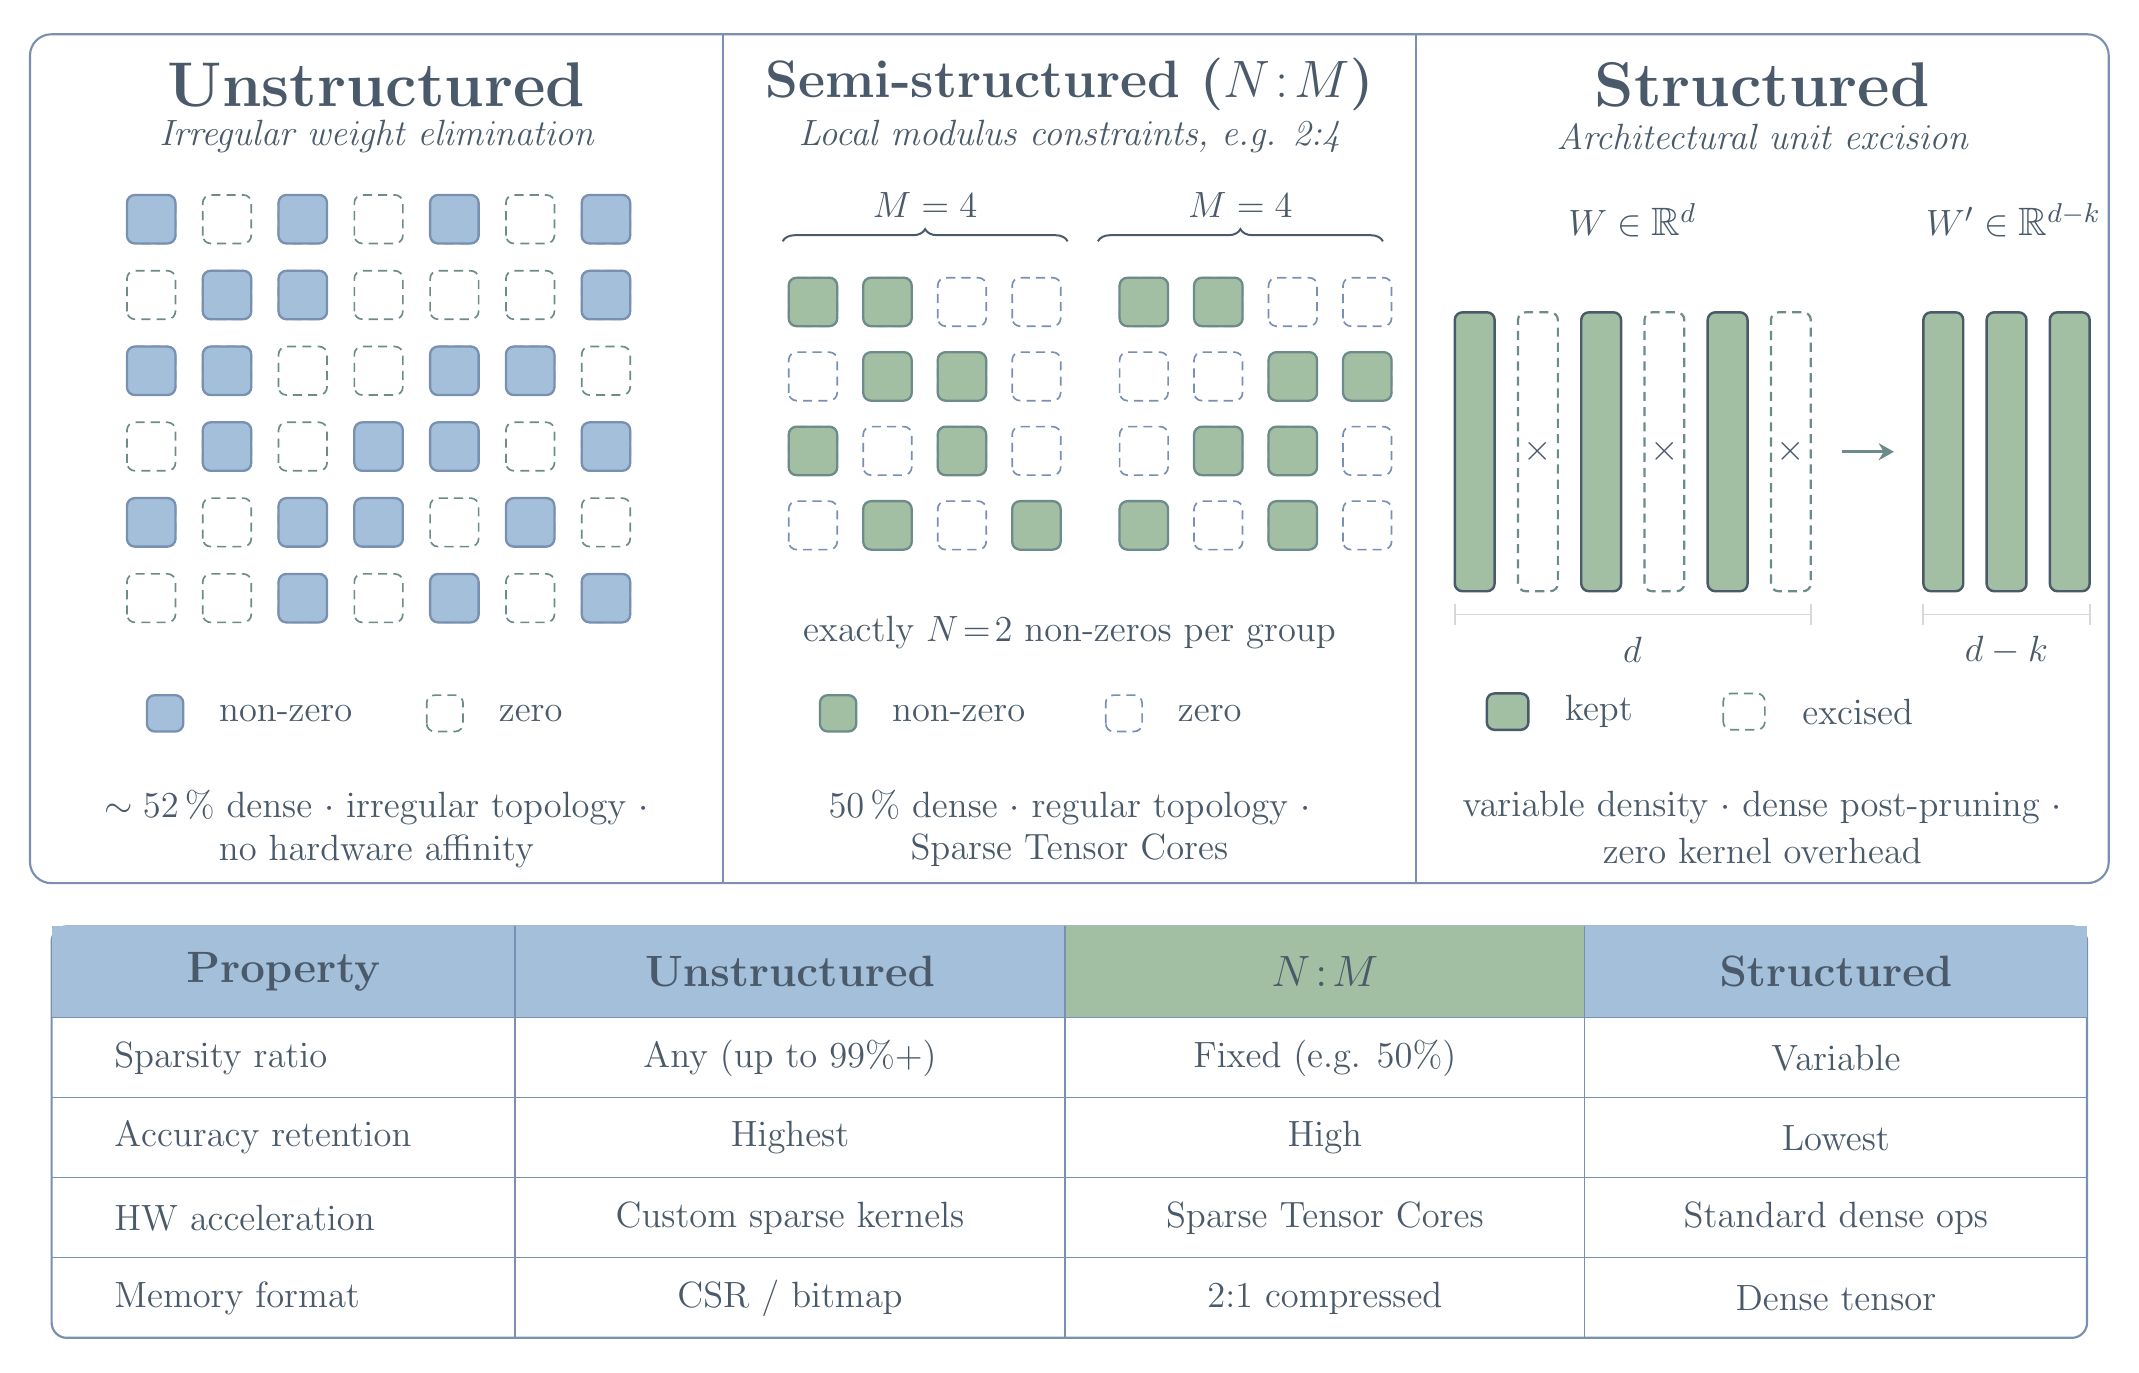
\includegraphics[width=0.92\linewidth]{pruning_topologies.png}
\caption{Sparsity topologies: unstructured, semi-structured ($N\!:\!M$),
and structured.}
\end{figure}
Only \textbf{structured} removal yields a smaller \emph{dense} network that runs
fast on standard kernels; unstructured zeros need sparse engines, and $2\!:\!4$
semi-structured sits in between (Ampere tensor cores).
\begin{table}
\renewcommand{\arraystretch}{1.25}
\small
\begin{tabularx}{\linewidth}{llX}
\toprule
\textbf{Arch.} & \textbf{Unit} & \textbf{Effect} \\
\midrule
MLP & Neuron & Hidden width \\
CNN & Filter & Feature maps \\
Transf. & Head & Attention diversity \\
Transf. & FFN channel & Intermediate width \\
Transf. & Layer & Depth \\
\bottomrule
\end{tabularx}
\caption{Structured units by architecture.}
\end{table}
\end{block}
\end{column}

\end{columns}

%---- full-width gold alert: the spine ----
\setbeamercolor{block alerted title}{fg=black,bg=dalgold}
\setbeamercolor{block alerted body}{fg=black,bg=white}
\begin{alertblock}{The Central Tension}
Almost every criterion scores each unit \textbf{locally and independently},
before the effect of the full set of removals is known. At high sparsity this
breaks down: a unit that looks redundant in isolation may become essential once
its neighbours are gone, and the way the budget is \emph{allocated across
layers} influences final quality more than any single local score. Sparsity
alone does not characterise a pruned network --- the configuration does.
\end{alertblock}

%---- full-width: strategies (wide pipeline figure) ----
\begin{block}{Pruning Strategies}
Strategy choice (\emph{when}, \emph{how often}, \emph{in what order} the mask is
updated) is largely orthogonal to criterion choice: \textbf{one-shot} (cheap,
errors compound), \textbf{iterative + recovery} (prune--finetune rounds on a
schedule), \textbf{during training} (dynamic sparse training, $\ell_1$), and
\textbf{post-training} (frozen model, calibration set only).
\begin{figure}
\resizebox{0.98\linewidth}{!}{%
\begin{tikzpicture}[
  font=\large,
  box/.style={rectangle, rounded corners=3pt, draw=colBlueBorder, fill=colBlue!15,
    minimum width=4.2cm, minimum height=1.1cm, align=center},
  data/.style={rectangle, rounded corners=3pt, draw=headergreen, fill=colGreen!25,
    minimum width=4.2cm, minimum height=1.1cm, align=center},
  arr/.style={-Stealth, very thick, colBlueBorder}]
  \node[data] (pretrain) {Pretrained\\$\Theta^\ast$};
  \node[data, right=1.1cm of pretrain] (calib) {Calibration\\($\le$512 samples)};
  \node[box, right=1.1cm of calib]  (stats) {Activation\\statistics};
  \node[box, right=1.1cm of stats]  (score) {Score units\\$S(\theta_i)$};
  \node[box, right=1.1cm of score]  (mask)  {Apply mask\\$M^\ast$};
  \node[box, right=1.1cm of mask]   (opt)   {(Optional)\\weight correction};
  \node[data, below=1.1cm of opt]   (pruned){Pruned model\\$M^\ast\!\odot\Theta^\ast$};
  \draw[arr] (pretrain) -- (stats);
  \draw[arr] (calib) -- (stats);
  \draw[arr] (stats) -- (score);
  \draw[arr] (score) -- (mask);
  \draw[arr] (mask) -- (opt);
  \draw[arr] (opt) -- (pruned);
\end{tikzpicture}}
\caption{Post-training pruning pipeline: no full retraining, only calibration
statistics and optional local weight correction (SparseGPT).}
\end{figure}
\end{block}

%---- bottom split: criteria | allocation ----
\begin{columns}[t,totalwidth=\twocolwid]

\begin{column}{\onecolwid}
\begin{block}{Pruning Criteria}
A criterion assigns an importance score as a proxy for the loss change of
removing a unit.
\begin{table}
\renewcommand{\arraystretch}{1.25}
\small
\begin{tabularx}{\linewidth}{lXc}
\toprule
\textbf{Criterion} & \textbf{Signal} & \textbf{Acc.} \\
\midrule
Magnitude & weights only & base \\
Gradient & grad $\times$ weight & +1--3\% \\
OBD & diag.\ curvature & +1--5\% \\
SparseGPT & per-layer $H^{-1}$ & best PT \\
Wanda & $|W|\!\cdot\!\norm{x}$ & strong PT \\
Movement & score trajectory & best FT \\
\bottomrule
\end{tabularx}
\caption{Criteria differ in the information used and the data/compute required;
gains are relative to magnitude pruning (PT = post-training, FT = fine-tune).}
\end{table}
\end{block}
\end{column}

\begin{column}{\onecolwid}
\begin{block}{Allocation Matters}
Layerwise (uniform $\kappa$) prunes sensitive and robust layers alike. Global
or sensitivity-guided allocation equalises the marginal loss impact across
layers.
\begin{figure}
\begin{tikzpicture}
\begin{axis}[
  ybar, bar width=8pt,
  width=0.98\linewidth, height=12cm,
  xlabel={Layer index}, ylabel={Loss increase at 50\% sparsity},
  xtick={1,3,5,7,9,11}, ymin=0, ymax=0.25,
  ymajorgrids=true, grid style={gray!20},
  legend pos=north west, legend style={font=\small}]
\addplot[fill=actred, draw=actreddark] coordinates {
 (1,0.19)(2,0.06)(3,0.04)(4,0.05)(5,0.03)(6,0.04)
 (7,0.05)(8,0.04)(9,0.06)(10,0.08)(11,0.12)(12,0.22)};
\addlegendentry{Attention}
\addplot[fill=colBlue!75!white, draw=colBlueBorder] coordinates {
 (1,0.12)(2,0.04)(3,0.03)(4,0.03)(5,0.02)(6,0.03)
 (7,0.03)(8,0.03)(9,0.04)(10,0.05)(11,0.09)(12,0.14)};
\addlegendentry{FFN}
\end{axis}
\end{tikzpicture}
\caption{Per-layer sensitivity (12-layer Transformer): first and last layers
are the most sensitive, so they deserve higher density.}
\end{figure}
\end{block}
\end{column}

\end{columns}

\end{column} % end column 2

\begin{column}{\sepwid}\end{column} % spacer

%========================================================================
% COLUMN 3
%========================================================================
\begin{column}{\onecolwid}

%---- Pruning transformers + architecture figure ----
\begin{block}{Pruning Transformers}
The removable units are not simple neurons: they are attention heads, FFN
channels, whole layers, and (dynamically) tokens.
\begin{figure}
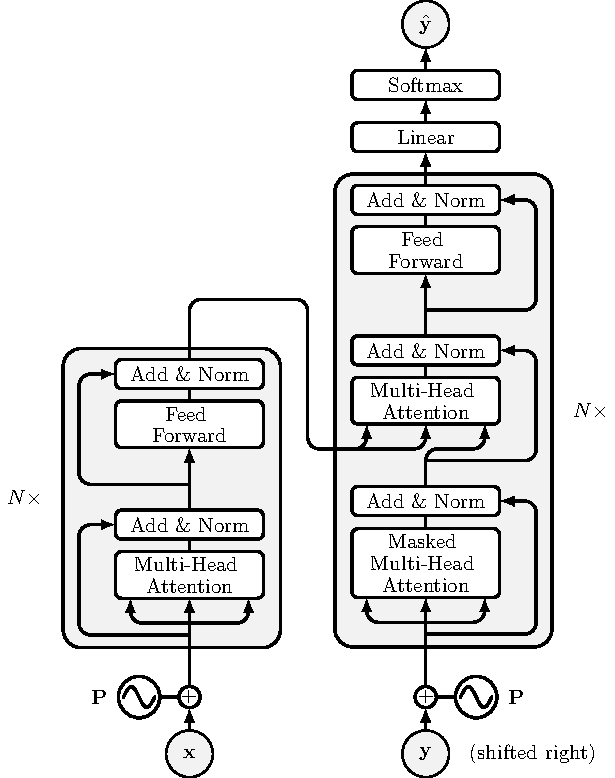
\includegraphics[width=0.66\linewidth]{transformer.pdf}
\caption{Encoder--decoder Transformer. Heads, FFN channels, and layers are the
structured pruning targets; tokens are pruned per input.}
\end{figure}
\begin{itemize}
\item \textbf{Head:} removes 4 matrices per head, $\Delta P=4d^2/H$; 20--40\% of
heads are often removable.
\item \textbf{FFN channel:} masks rows of $W_1$ and columns of $W_2$; entangled
under SwiGLU.
\item \textbf{Layer:} drops a residual block by its contribution
$\norm{F_l(X)}/\norm{X}$; cheap depth, costly capacity.
\item \textbf{Token:} input-dependent; targets the $O(T^2)$ attention cost.
\end{itemize}
\end{block}

%---- Results: search-based at high compression ----
\begin{block}{Results: Search at High Compression}
WikiText-2 / C4 perplexity ($\downarrow$). Global allocation search (EvoPress)
versus block-scoring depth pruning (ShortGPT) and uniform allocation.
\begin{table}
\centering
\renewcommand{\arraystretch}{1.25}\small
\begin{tabular}{llrr}
\toprule
\textbf{Model / Budget} & \textbf{Method} & \textbf{Wiki2} & \textbf{C4} \\
\midrule
Mistral-7B, 25\%   & EvoPress & \textbf{8.66}  & \textbf{12.04} \\
                   & ShortGPT & 43.26 & 40.16 \\
Llama-2-7B, 37.5\% & EvoPress & \textbf{17.98} & \textbf{18.91} \\
                   & ShortGPT & 70.94 & 63.51 \\
Mistral-7B, 70\%   & EvoPress & \textbf{14.42} & \textbf{16.46} \\
                   & Uniform  & 23.08 & 30.03 \\
\bottomrule
\end{tabular}
\caption{At aggressive budgets, global configuration search dominates local
block scoring and uniform allocation by large margins.}
\end{table}
\end{block}

%---- Discussion ----
\begin{block}{Discussion}
\begin{itemize}
\item \textbf{Local vs.\ global.} Criteria such as SparseGPT and Wanda score
units \emph{before} the compressed model is fixed; they identify removable
weights but do not decide how to distribute the budget across layers.
\item \textbf{High-compression limit.} Local ranking assumes removals are
independent, but residual and attention structure couple layers --- so
allocation search (ZipLM, EvoPress) becomes the dominant factor.
\item \textbf{Comparability.} Reported gains span five evaluation regimes and
very different recovery budgets (Fisher $\approx$39\,s vs.\ CoFi 40 epochs);
post-training methods are also calibration-sensitive.
\end{itemize}
\end{block}

%---- References ----
\begin{block}{Key References}
\small
\begin{itemize}
\item LeCun et al., \emph{Optimal Brain Damage}, 1989.
\item Hassibi \& Stork, \emph{Optimal Brain Surgeon}, 1993.
\item Frankle \& Carbin, \emph{Lottery Ticket Hypothesis}, 2019.
\item Frantar \& Alistarh, \emph{SparseGPT}, 2023.
\item Sun et al., \emph{Wanda}, 2023.
\item Sanh et al., \emph{Movement Pruning}, 2020.
\end{itemize}
\end{block}

%---- Contact ----
\setbeamercolor{block alerted title}{fg=black,bg=dalblue}
\setbeamercolor{block alerted body}{fg=black,bg=white}
\begin{alertblock}{Contact}
\begin{itemize}
\item Email: [your.email@university.edu]
\item Thesis: \emph{Transformer Compression}
\end{itemize}
\end{alertblock}

\begin{center}

\includegraphics[width=0.5\linewidth]{dal_fullmark_blak.png}
\end{center}

\end{column} % end column 3

\end{columns}
\end{frame}
\end{document}
